\documentclass{article}

\usepackage[solutions]{xrcise}

\begin{document}
\sheet[2021]{Ersttermin}
\begin{exercise}{Kruskal-Algorithmus}
  Betrachten Sie den Graphen in \ref{fig:kruskal2021}. Bestimmen Sie mit Hilfe des Algorithmus von Kruskal einen minimalen Spannbaum des Graphen und skizzieren diesen. Geben Sie zusätzlich die Reihenfolge an, in der die Kanten des Spannbaums gemäß Algorithmus hinzugefügt werden.
  \begin{figure}
  \centering
  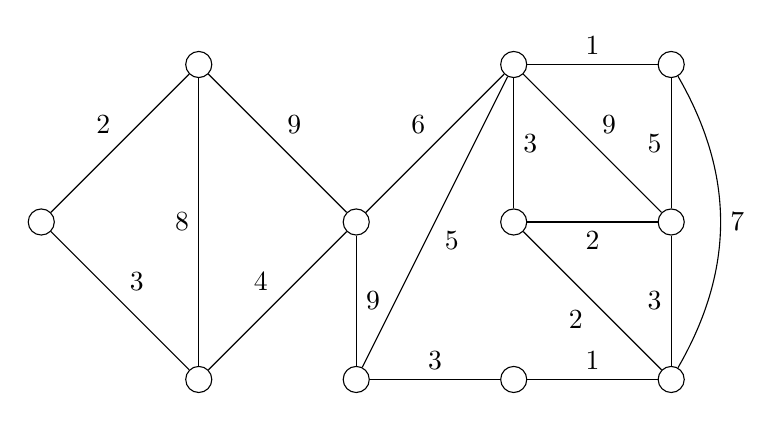
\begin{tikzpicture}[auto, node distance=2cm, main node/.style={circle, draw, minimum size=.5em}]
    \node[main node] (0) {};
    \node[main node] (1) [right of=0, below of=0] {};
    \node[main node] (2) [above of=1, above of=1] {};
    \node[main node] (3) [right of=2, below of=2] {};
    \node[main node] (4) [right of=3, above of=3] {};
    \node[main node] (5) [right of=4] {};
    \node[main node] (6) [below of=3] {};
    \node[main node] (7) [right of=6] {};
    \node[main node] (8) [right of=7] {};
    \node[main node] (9) [above of=8] {};
    \node[main node] (10) [left of=9] {};

    \path[every node]
    (0) edge node {3} (1)
    (0) edge node {2} (2)
    (1) edge node {8} (2)
    (1) edge node {4} (3)
    (2) edge node {9} (3)
    (3) edge node {6} (4)
    (3) edge node {9} (6)
    (4) edge node {1} (5)
    (4) edge node {5} (6)
    (4) edge node {9} (9)
    (4) edge node {3} (10)
    (5) edge[bend left] node {7} (8)
    (9) edge node {5} (5)
    (6) edge node {3} (7)
    (7) edge node {1} (8)
    (8) edge node {3} (9)
    (8) edge node {2} (10)
    (9) edge node {2} (10)
    ;
  \end{tikzpicture}

  \caption{Ein gewichteter Graph}\label{fig:kruskal}
\end{figure}

  \begin{solution}
    \begin{figure}
  \centering
  \begin{tikzpicture}[auto,on grid, node distance=2cm, vertex/.style={circle, draw, minimum size=0.75cm}]
    \node[vertex] (a) {a};
    \node[vertex, right=of a] (b) {b};
    \node[vertex, right=of b] (c) {c};
    \node[vertex, right=of c] (d) {d};
    \node[vertex, right=of d] (e) {e};
    \node[vertex, below right=2cm and 1cm of a] (f) {f};
    \node[vertex, right=of f] (g) {g};
    \node[vertex, right=of g] (h) {h};
    \node[vertex, right=of h] (i) {i};

    \draw (a) -- node {17{\tiny(6)}} (b);
    \draw (c) -- node {5{\tiny(3)}} (d);
    \draw (e) -- node {13{\tiny(5)}} (i);
    \draw (i) -- node {19{\tiny(7)}} (h);
    \draw (h) -- node {7{\tiny(4)}} (g);
    \draw (g) -- node {23{\tiny(8)}} (f);
    \draw (b) -- node {3{\tiny(2)}} (f);
    \draw (d) -- node {2{\tiny(1)}} (h);
  \end{tikzpicture}

  \caption{Ein minimaler Spannbaum zu \ref{fig:kruskal2021}.}\label{fig:kruskal2021solution}
\end{figure}
  \end{solution}
\end{exercise}

\begin{exercise}{AVL-Bäume}
  Gegeben sei ein AVL-Baum für die Schlüssel $\{2,3,5,7,11,13,17,19\}$. Der Zustand der Datenstruktur ist in \ref{fig:avl} dargestellt. Skizzieren Sie die Datenstruktur nach dem Einfügen eines Elements mit Schlüssel 6 gemäß der Einfügeoperation aus der Vorlesung. Machen Sie dabei den jeweiligen Zustand vor und nach eventuell notwendigen Balancierungsschritten deutlich.
  \begin{figure}
  \centering
  \begin{tikzpicture}[auto,on grid,node distance=2cm,main node/.style={circle,draw,minimum size=0.75cm}]
    \node[main node] (5) {5};
    \node[main node, below left=of 5] (3) {3};
    \node[main node, below left=of 3] (2) {2};
    \node[main node, below right=of 5] (17) {17};
    \node[main node, below left=of 17] (11) {11};
    \node[main node, below right=of 17] (19) {19};
    \node[main node, below left=of 11] (7) {7};
    \node[main node, below right=of 11] (13) {13};

    \draw (5) -- (3) -- (2);
    \draw (5) -- (17) -- (11) -- (7);
    \draw (17) -- (19);
    \draw (11) -- (13);
  \end{tikzpicture}

  \caption{AVL-Baum für die Schlüssel $2, 3, 5, 7, 11, 13, 17, 19$.}\label{fig:avl}
\end{figure}

  \begin{solution}
    \begin{figure}
  \centering
  \begin{tikzpicture}[auto,on grid,node distance=2cm,main node/.style={circle,draw,minimum size=0.75cm}]
    \node[main node] (5) {5};
    \node[main node, below left=of 5] (3) {3};
    \node[main node, below left=of 3] (2) {2};
    \node[main node, below right=of 5] (17) {17};
    \node[main node, below left=of 17] (11) {11};
    \node[main node, below right=of 17] (19) {19};
    \node[main node, below left=of 11] (7) {7};
    \node[main node, below right=of 11] (13) {13};
    \node[main node, below left=of 7] (6) {6};

    \draw (5) -- (3) -- (2);
    \draw (5) -- (17) -- (11) -- (7);
    \draw (17) -- (19);
    \draw (11) -- (13);
    \draw (7) -- (6);
  \end{tikzpicture}

  \caption{AVL-Baum nach dem Einfügen von $6$}\label{fig:avlsolution1}
\end{figure}

\begin{figure}
  \centering
  \begin{tikzpicture}[auto,on grid,node distance=2cm,main node/.style={circle,draw,minimum size=0.75cm}]
    \node[main node] (5) {5};
    \node[main node, below left=of 5] (3) {3};
    \node[main node, below left=of 3] (2) {2};
    \node[main node, below right=of 5] (11) {11};
    \node[main node, below left=of 11] (7) {7};
    \node[main node, below right=of 11] (17) {17};
    \node[main node, below right=of 17] (19) {19};
    \node[main node, below right=of 7] (13) {13};
    \node[main node, below left=of 7] (6) {6};

    \draw (5) -- (3) -- (2);
    \draw (5) -- (11) -- (17) -- (19);
    \draw (11) -- (7) -- (6);
    \draw (17) -- (13);
  \end{tikzpicture}

  \caption{Balancierter AVL-Baum nach Rotation}\label{fig:avlsolution}
\end{figure}
  \end{solution}
\end{exercise}

\begin{exercise}{Big-O Notation}
  Jede der folgenden Teilaufgaben spezifiziert zwei Funktionen $f(n)$ und $g(n)$. Bestimmen Sie jeweils, ob die vier Relationen $f(n) = o(g(n))$, $f(n) = O(g(n))$, $f(n) = \Omega(g(n))$ und $f(n) = \omega(g(n))$ gelten (es sind also pro Teilaufgabe vier Antworten zu geben). Beweisen Sie Ihre Antwort jeweils kurz. Nutzen Sie dazu die Eigenschaften der asymptotischen Landau-Notation aus der Vorlesung (wie z. B. die Charakterisierung über Grenzwerte).
  \begin{enumerate}
    \item $f(n) = n \cdot (\log n)^{42}$ und $g(n) = n^{1.23}$
    \item $f(n) = n \cdot |\sin n|$ und $g(n) = \sqrt{n}$
    \item $f(n) = n^2 + n^{3/2} + n \cdot \log n$ und $g(n) = \binom{n}{2}$
    \item $f(n) = 8^{\log n}$ und $g(n) = n^3 \cdot \log n$
  \end{enumerate}
  \hint{Der Ausdruck $\binom{n}{k}$ bezeichnet den Binomialkoeffizienten $n$ über $k$. Die Basis des Logarithmus in Ausdrücken der Form $\log n$ ist 2.}

  \begin{solution}
    \begin{enumerate}
      \item Da Logarithmen generell langsamer wachsen als polynomielle Funktionen, ergibt sich für die Grenzwerte: \[
              \lim_{n \to \infty} \frac{n \cdot (\log n)^{42}}{n^{1.23}} = \lim_{n \to \infty} \frac{(\log n)^{42}}{n^{0.23}} = 0
            \]
            Also gilt $f(n) = o(g(n))$ und $f(n) = O(g(n))$. $f(n) = \Omega(g(n))$ und $f(n) = \omega(g(n))$ gelten nicht.
      \item Da $|\sin n| \in [0\dots1]$ für alle $n \in \mathbb{N}$, ergibt sich für die Grenzwerte: \[
              \lim_{n \to \infty} \frac{n \cdot |\sin n|}{\sqrt{n}} = \lim_{n \to \infty} \sqrt{n} \cdot |\sin n| = [0\dots\infty]
            \]
            Es gilt keine der Relationen, da der Grenzwert weder größer null noch kleiner unendlich ist (Je nach Ausprägung von $|\sin n|$).
      \item Da $\binom{n}{2} = \frac{n \cdot (n-1)}{2}$, ergibt sich für die Grenzwerte: \[
              \lim_{n \to \infty} \frac{n^2 + n^{3/2} + n \cdot \log n}{\frac{n \cdot (n-1)}{2}} = \lim_{n \to \infty} \frac{\Theta(n^2)}{\Theta(n^2)} = \Theta(1)
            \]
            Es gelten $f(n) = \Omega(g(n))$ und $f(n) = \bigO(g(n))$, da der Grenzwert größer null und kleiner unendlich ist. $f(n) = o(g(n))$ und $f(n) = \omega(g(n))$ gelten nicht.
      \item Da $f(n) = 8^{\log n} = (2^3)^{\log n} = 2^{3 \cdot \log n} = n^3$, ergibt sich für die Grenzwerte: \[
              \lim_{n \to \infty} \frac{8^{\log n}}{n^3 \cdot \log n} = \lim_{n \to \infty} \frac{n^3}{n^3 \cdot \log n} = \lim_{n \to \infty} \frac{1}{\log n} = 0
            \]
            Also gilt $f(n) = o(g(n))$ und $f(n) = O(g(n))$. $f(n) = \Omega(g(n))$ und $f(n) = \omega(g(n))$ gelten nicht.
    \end{enumerate}
  \end{solution}
\end{exercise}

\begin{exercise}{Union-Find Datenstruktur}
  Wir betrachten die Datenstruktur für disjunkte dynamische Mengen wie in der Vorlesung definiert. Die Grundmenge (das Universum) sei $U = \{a, b, . . . , z\}$, also die Menge der 26 Kleinbuchstaben $a$ bis $z$.
  \begin{enumerate}
    \item\label{ex:unionFind:1} Geben Sie eine Folge von Aufrufen der Operationen \textalgo{MakeSet} und \textalgo{Union} an, welche die disjunkten Mengen $S_1 = \{a\}$, $S_2 = \{b, c, d\}$ sowie $S_3 = \{e, f\}$ erzeugt.
    \item Skizzieren Sie die Mengenobjekte der Datenstruktur, nachdem die disjunkten Mengen gemäß Ihrer Lösung zu Punkt (a) erzeugt wurden. Eine mögliche Darstellung ist in \ref{fig:unionFind} zu sehen.
    \item Geben Sie jeweils den Rückgabewert des Aufrufes \textalgo{FindSet(a)} und des Aufrufes \textalgo{FindSet(d)} an, nachdem die disjunkten Mengen gemäß Ihrer Lösung zu Punkt (a) erzeugt wurden.
    \item Skizzieren Sie das Mengenobjekt, welches entsteht, wenn nach Ihrer Lösung aus \ref{ex:unionFind:1} die Operation \textalgo{Union(c,f)} ausgeführt wird. Nutzen Sie wieder eine Darstellung ähnlich zu \ref{fig:unionFind}.
  \end{enumerate}
  \begin{figure}
  \centering
  \includegraphics[width=0.5\textwidth]{res/unionFind}

  \caption{Union-Find Datenstruktur}\label{fig:unionFind}
\end{figure}

  \begin{solution}
    \begin{enumerate}
      \item Die Folge von Aufrufen ist:\par
            \textalgo{MakeSet(a)}, \textalgo{MakeSet(b)}, \textalgo{MakeSet(c)}, \textalgo{MakeSet(d)}, \textalgo{MakeSet(e)}, \textalgo{MakeSet(f)},\par
            \textalgo{Union(b, c)}, \textalgo{Union(b, d)}, \textalgo{Union(e, f)}.
      \item Skizze: \begin{figure}
  \begin{tabular}{ccc}
    \begin{tikzpicture}[->, auto, on grid, node distance=2cm, every node/.style={rectangle, draw}]
      \node (head) {head};
      \node[below=1cm of head] (tail) {tail};
      \node[right=of head] (a) {a};

      \node[style={draw=none}, below left=.5cm and 1cm of head] (s) {$S_1$};

      \draw (head) -- (a);
      \draw (tail) -| (a);
      \draw (a) -- +(0,1) -| (head);
    \end{tikzpicture} &

    \begin{tikzpicture}[->, auto, on grid, node distance=2cm, every node/.style={rectangle, draw}]
      \node (head) {head};
      \node[below=1cm of head] (tail) {tail};
      \node[right=of head] (b) {b};
      \node[right=of b] (c) {c};
      \node[right=of c] (d) {d};

      \node[style={draw=none}, below left=.5cm and 1cm of head] (s) {$S_2$};

      \draw (head) -- (b);
      \draw (b) -- (c);
      \draw (c) -- (d);
      \draw (tail) -| (d);
      \draw (b) -- +(0,.5) -| (head);
      \draw (c) -- +(0,.75) -| (head);
      \draw (d) -- +(0,1) -| (head);
    \end{tikzpicture} &

    \begin{tikzpicture}[->, auto, on grid, node distance=2cm, every node/.style={rectangle, draw}]
      \node (head) {head};
      \node[below=1cm of head] (tail) {tail};
      \node[right=of head] (e) {e};
      \node[right=of e] (f) {f};

      \node[style={draw=none}, below left=.5cm and 1cm of head] (s) {$S_3$};

      \draw (head) -- (e);
      \draw (e) -- (f);
      \draw (tail) -| (f);
      \draw (e) -- +(0,.75) -| (head);
      \draw (f) -- +(0,1) -| (head);
    \end{tikzpicture}
  \end{tabular}

  \caption{Das Mengenobjekt der Datenstruktur nach Ausführung der Operationen}\label{fig:unionFindSolution}
\end{figure}
      \item \textalgo{FindSet(a)} gibt $a$ zurück und \textalgo{FindSet(d)} gibt $b$ zurück.
      \item Skizze: \begin{figure}
  \centering
  \begin{tikzpicture}[->, auto, on grid, node distance=2cm, every node/.style={rectangle, draw}]
    \node (head) {head};
    \node[below=1cm of head] (tail) {tail};
    \node[right=of head] (b) {b};
    \node[right=of b] (c) {c};
    \node[right=of c] (d) {d};
    \node[right=of d] (e) {e};
    \node[right=of e] (f) {f};

    \draw (head) -- (b);
    \draw (b) -- (c);
    \draw (c) -- (d);
    \draw (d) -- (e);
    \draw (e) -- (f);
    \draw (tail) -| (f);
    \draw (b) -- +(0,.25) -| (head);
    \draw (c) -- +(0,.5) -| (head);
    \draw (d) -- +(0,.75) -| (head);
    \draw (e) -- +(0,1) -| (head);
    \draw (f) -- +(0,1.25) -| (head);
  \end{tikzpicture}

  \caption{Das Mengenobjekt der Datenstruktur nach Operation \textalgo{Union(c,f)}}\label{fig:unionFindSolution2}
\end{figure}
    \end{enumerate}
  \end{solution}
\end{exercise}

\begin{exercise}{Divide \& Conquer}
  Betrachten Sie den Divide \& Conquer Algorithmus, dessen Pseudocode in \ref{alg:Algo} gegeben ist und lösen Sie folgende Aufgaben:
  \begin{enumerate}
    \item Geben Sie eine Rekursionsgleichung für die Laufzeit $T(n)$ des Algorithmus bei Eingabe $(A, 1, n)$ für ein Array $A$ der Länge $n \in \mathbb{N}$ an.
    \item Analysieren Sie die Laufzeit von Algorithmus 1 möglichst genau in der $O$-Notation mit Hilfe der Substitutionsmethode. Sie können dabei annehmen, dass $n$ eine Zweierpotenz ist.
  \end{enumerate}
  \hint{Ein Induktionsbeweis der Laufzeit ist nicht notwendig, aber aus Ihrer Rechnung muss klar hervorgehen, wie Sie zu Ihrer Lösung kommen.}
  \begin{alg}
  % Algo(A, l, r)
  % n←r−l+1 ifn≤2
  % ifn=2
  % return |A[r] − A[l]|
  % else return 0 else
  % p←⌊(l+r)/2⌋
  % a ← Algo(A, l, p) b←Algo(A,p+1,r) ifa>b
  % c←a else c←b
  % fori←ltop
  % for j ← p + 1 to r
  % Lösung
  % (a)
  % Algorithmus 1
  % (Θ(1)
  % 2T (n/2) + Θ(n2)
  % return c
  % x ← |A[i] − A[j]| if x > c
  % c←x

\end{alg}

  \begin{solution}
    \begin{enumerate}
      \item Die Rekursionsgleichung ist: \[
              T(n) = \begin{cases}
                \Theta(1),                    & \text{falls } n \leq 2, \\
                2 \cdot T(n/2) + \Theta(n^2), & \text{sonst}.
              \end{cases}
            \]
      \item Die Lösung der Rekursionsgleichung ist: \[
              T(n) = \Theta(n^2).
            \]
    \end{enumerate}
  \end{solution}
\end{exercise}

\begin{exercise}{Datenstrukturen}
  Gesucht ist eine Datenstruktur, welche die drei folgenden Operationen unterstützt:
  \begin{itemize}
    \item \textalgo{Einfügen}(x): Fügt die Zahl x in die Datenstruktur ein. Sie können zur Vereinfachung davon ausgehen, dass kein Element jemals doppelt in die Datenstruktur eingefügt wird.
    \item \textalgo{Löschen}(x): Entfernt x, falls sich x in der Datenstruktur befindet. Andernfalls bleibt die Datenstruktur unverändert.
    \item \textalgo{Rang}(x): Gibt die Anzahl der Elemente der Datenstruktur zurück, welche kleiner oder gleich x sind. Befinden sich z. B. die Zahlen $\{2,3,5,7,11,13\}$ in der Datenstruktur, so soll $Rang(5) = 3$ und $Rang(17) = 6$ gelten.
  \end{itemize}
  Die Datenstruktur soll alle drei Operationen in Laufzeit $O(\log n)$ unterstützen. Dabei bezeichnet $n$ die Anzahl der Elemente, die sich aktuell in der Datenstruktur befinden.\par
  Beschreiben Sie in wenigen kurzen Sätzen, wie Ihre Datenstruktur aufgebaut ist und wie die angegebenen Operationen realisiert werden. Hierbei ist kein Pseudocode gefordert. Es soll jedoch klar werden, dass die Datenstruktur korrekt arbeitet und die geforderte Laufzeit eingehalten wird.

  \begin{solution}
    Es bietet sich ein modifizierter AVL-Baum an. Jeder Knoten speichert zusätzlich die Anzahl der Elemente in seinem linken und rechten Teilbaum.\par
    Die Operationen \textalgo{Einfügen} und \textalgo{Löschen} werden wie bei einem normalen AVL-Baum durchgeführt und die Größeninformationen werden entsprechend aktualisiert.\par
    Die Operation \textalgo{Rang} wird durch eine Suche im Baum realisiert, wobei die Größeninformationen der Teilbäume genutzt werden, um die Anzahl der Elemente zu bestimmen, die kleiner oder gleich x sind.
  \end{solution}
\end{exercise}

\begin{exercise}{Dynamische Programmierung}
  Ein Unternehmen erhält die Genehmigung, eine Landstraße auf einer Straßenseite mit Werbetafeln zu versehen. Entlang der $n \in \mathbb{N}$ Kilometer langen Landstraße gibt es im Abstand von je genau einem Kilometer $n + 1$ geeignete Standorte. Für den Standort bei Kilometer $i \in \{0,1,...,n\}$ sind Werbekunden bereit, einen Betrag $w_i > 0$ an das Unternehmen zu zahlen. Allerdings besagt die Straßenverkehrsordnung, dass zwischen je zwei Werbetafeln mindestens zwei Kilometer Abstand bestehen müssen. Errichtet das Unternehmen also bei Kilometer $i$ eine Werbetafel, so darf bei Kilometer $i - 1$ und $i + 1$ keine Werbetafel errichtet werden. Helfen Sie dem Unternehmen anhand der folgenden Schritte eine Auswahl an Standorten zu bestimmen, die den Gesamtgewinn aus der Vermietung der Standorte maximiert.
  \begin{enumerate}
    \item Für $k \in \{0, 1, \dots, n\}$ bezeichne $\text{OPT}(k)$ den maximal erzielbaren Gesamtgewinn, wenn das Unternehmen nur die Standorte an den Kilometern $0,1,...,k$ für die Errichtung von Werbetafeln in Betracht zieht. Finden Sie eine rekursive Formulierung für $\text{OPT}(k)$ und begründen Sie kurz deren Korrektheit.
    \item Bezeichne $W[0..n]$ ein Array der Länge $n + 1$, so dass $W[i] = w_i$ dem Eintrag des Standortes bei Kilometer $i$ entspricht. Beschreiben Sie in Pseudocode einen Algorithmus, der mittels dynamischer Programmierung bei Eingabe $(W, n)$ in Zeit $O(n)$ den maximalen Gesamtgewinn, den das Unternehmen erzielen kann, ermittelt. Die Liste der Standorte, die dieses Maximum erreicht, muss nicht bestimmt werden.
  \end{enumerate}

  \begin{solution}
    \begin{enumerate}
      \item Die rekursive Formulierung ist: \[
              \text{OPT}(k) = \begin{cases}
                0,                                              & \text{falls } k = 0, \\
                w_k,                                            & \text{falls } k = 1, \\
                \max\{w_k + \text{OPT}(k-2), \text{OPT}(k-1)\}, & \text{sonst}.
              \end{cases}
            \]
            Die Korrektheit der Formulierung ergibt sich aus der Tatsache, dass der maximale Gewinn entweder durch die Errichtung einer Werbetafel bei Kilometer $k$ oder durch die Nicht-Errichtung einer Werbetafel bei Kilometer $k$ erreicht wird.
      \item Ein Algorithmus könnte folgendermaßen funktionieren: \begin{alg}
  \signed{MaxGewinn}{W, n}{x}
  \params{Ein Array $W$ der Länge $n + 1$ und eine natürliche Zahl $n$.}{Der maximale Gesamtgewinn, den das Unternehmen erzielen kann.}

  $M[0] \gets 0$ \\
  $M[1] \gets W[1]$ \\
  \For{$k \gets 2$ \KwTo $n$}{
    $M[k] \gets \max\{W[k] + M[k-2], M[k-1]\}$
  }
  \Return{$M[n]$}
\end{alg}
    \end{enumerate}
  \end{solution}
\end{exercise}

\begin{exercise}{Greedy-Algorithmen}
  Das Tankstopp-Problem modelliert die folgende Situation: Auf der Autofahrt von Ihrem Startpunkt $t_0$ bis zu Ihrem Ziel $t_n$ wollen Sie so wenige Tankstopps wie möglich einlegen. Unterwegs kommen Sie der Reihe nach an den Tankstellen $t_1,t_2,...,t_{n-1}$ vorbei. Sie starten mit vollem Tank und eine Tankfüllung Ihres Wagens reicht für $D$ Kilometer. Der Abstand zwischen den Tankstellen $t_{i-1}$ und $t_i$ beträgt $d_i$ Kilometer, wobei $0 < d_i \leq D$ gilt. Betrachten Sie die folgende Greedy-Strategie:
  \begin{quote}
    Fahre stets so weit wie möglich ohne Tankstopp und tanke erst an der am weitesten entfernten noch erreichbaren Tankstelle voll.
  \end{quote}
  Beweisen Sie, dass diese Greedy-Strategie eine optimale Lösung liefert, die Anzahl der Tankstopps also minimal ist.
  \hint{Die Lösung einer Strategie $A$, die $k$ Tankstopps benötigt, kann zum Beispiel als Folge von Indizes $a(1) < a(2) < \dots < a(k)$ mit $a(i) \in \{1,2,...,n\}$ beschrieben werden. Der $i$-te Tankstopp findet dabei an der Tankstelle $t_{a(i)}$ statt.}

  \begin{solution}
    Wir beweisen die Aussage durch Widerspruch. Angenommen, es gibt eine optimale Lösung $A$, die mehr Tankstopps benötigt als die Greedy-Strategie. Sei $a(1) < a(2) < \dots < a(k)$ die Lösung $A$ und $b(1) < b(2) < \dots < b(l)$ die Lösung der Greedy-Strategie. Sei $i$ der kleinste Index, für den $a(i) \neq b(i)$ gilt. Dann gilt $a(i) > b(i)$, da die Greedy-Strategie immer so weit wie möglich fährt. Da $a(i) > b(i)$, gibt es eine Tankstelle $t_j$ mit $j < a(i)$, die in der Lösung $A$ nicht angesteuert wird. Da die Tankstelle $t_j$ in der Lösung $A$ nicht angesteuert wird, kann die Tankstelle $t_{a(i)}$ in der Lösung $A$ nicht erreicht werden, ohne dass ein Tankstopp eingelegt wird. Dies ist ein Widerspruch zur Annahme, dass $A$ eine optimale Lösung ist.
  \end{solution}
\end{exercise}

\begin{exercise}{NP-Vollständigkeit}
  Im Folgenden definieren wir zwei Entscheidungsprobleme:
  \begin{itemize}
    \item \textproblem{Unabhängige Menge}: Eine unabhängige Menge eines ungerichteten Graphen $G = (V,E)$ ist eine Teilmenge von Knoten $U \subseteq V$, so dass keine zwei Knoten aus $U$ adjazent sind. Es gilt also $\{u,v\} \in E$ für alle $u,v \in U$ mit $u \neq v$. Im Entscheidungsproblem \textproblem{Unabhängige Menge} ist ein kodiertes Paar $\langle G, k \rangle$ gegeben, wobei $G = (V,E)$ ein ungerichteter Graph ist und $k \in \mathbb{N}$. Es muss entschieden werden, ob $G$ eine unabhängige Menge $U \subseteq V$ der Größe $|U| \geq k$ enthält. Abbildung 4a zeigt ein Beispiel für eine Instanz des Problems.
    \item \textproblem{Keine Schnitte}: Gegeben ist ein kodiertes Paar $\langle S, l \rangle$, wobei $S = \{I_1, I_2, \dots\}$ eine endliche Menge von Intervallen $I_i \subseteq \mathbb{R}$ ist und $l \in \mathbb{N}$. Es muss entschieden werden, ob es eine Teilmenge $T \subseteq S$ von $S$ der Größe $|T| \geq l$ gibt, so dass alle Intervalle in $T$ paarweise disjunkt sind.
  \end{itemize}
  \hint{Sie dürfen zur Lösung der folgenden Aufgaben benutzen, dass \textproblem{Unabhängige Menge} NP-schwer ist.}
  \begin{enumerate}
    \item Ist \textproblem{Unabhängige Menge} NP-vollständig? Beweisen Sie Ihre Antwort.
    \item Beweisen Sie \textproblem{Keine Schnitte} $\leq_P$ \textproblem{Unabhängige Menge}.
    \item Was folgt daraus für die Komplexität von \textproblem{Keine Schnitte}?
  \end{enumerate}

  \begin{solution}
    \begin{enumerate}
      \item Eine Lösung von \textproblem{Unabhängige Menge} kann in P überprüft werden, indem für jedes Paar von Knoten in der unabhängigen Menge geprüft wird, ob es eine Kante zwischen den beiden Knoten gibt. Dieser Schritt benötigt Zeit $O(V^2)$, was in P liegt. Daher ist \textproblem{Unabhängige Menge} in NP. Da es annahmegemäß NP-schwer ist, folgt aus der Definition von NP-Vollständigkeit, dass \textproblem{Unabhängige Menge} NP-vollständig ist.
      \item Wir reduzieren \textproblem{Keine Schnitte} auf \textproblem{Unabhängige Menge}, indem wir für jedes Intervall $I_i \in S$ einen Knoten $v_i$ in einem Graphen $G$ erzeugen. Dann fügen wir eine Kante zwischen $v_i$ und $v_j$ hinzu, wenn die Intervalle $I_i$ und $I_j$ nicht disjunkt sind. Das Ergebnis ist ein Graph $G = (V,E)$, wobei $V = \{v_1, v_2, \dots\}$ und $E \subseteq V \times V$. Dann ist $\langle S, l \rangle$ eine Instanz von \textproblem{Keine Schnitte} genau dann, wenn $\langle G, l \rangle$ eine Instanz von \textproblem{Unabhängige Menge} ist.
      \item Da \textproblem{Unabhängige Menge} NP-vollständig ist, folgt aus der Reduktion \textproblem{Keine Schnitte} $\leq_P$ \textproblem{Unabhängige Menge}, dass \textproblem{Keine Schnitte} NP-vollständig ist.
    \end{enumerate}
  \end{solution}
\end{exercise}
\end{document}